\chapter[Accommodation Module for Spoken Dialogue Systems]{Accommodation Module for\\Spoken Dialogue Systems}
\label{chap:convergence_module_for_sdss}

\lettrine{T}{his} chapter introduces a plug-and-use module for \acs{sds} that adds support for vocal accommodation.
It is integrated into the system as a new link between the \acs{asr} and \acs{tts} modules.
The implementation and integration details as well as a demonstration of manipulating the system's output using this module are presented and discussed.

\pagebreak

\section{Modularization}
\label{sec:modularization}

An implementation of the pipeline introduced in \cref{sec:pipeline_representation} is presented here as an independent module for \acp{sds}.
It is shown how the statistical components from \cref{chap:statistical_model} can be added to it to take advantage of the capabilities of both approaches.
While supra-segmental features can be handled as well, only segmental features are discussed here, as they are less represented in accommodation modeling works and they require additional considerations, like segment context and local manipulation, as demonstrated in this chapter \citep[as explained in][]{Raveh2017SemDial}.
Thanks to the independence of this module, it can be added into any existing system that can provide the user's speech signal as input and a \ac{tts} module that can receive its output.
The \ac{sds} presented in \cref{chap:web-based_responsive_spoken_dialogue_system} has this module integrated into it to generate accommodative behaviors.

\subsection{Accommodation pipeline}
\label{subsec:computational_model}

The implementations of the pipeline's steps will be explained using the feature definition with the properties described in \cref{tab:feature_definition}.
%
\begin{table}[t]
	\centering
	\caption[Feature definition example]
		{Example of a feature definition used in the pipeline.
		 The definition described  the feature \emph{\textipa{@}-length}, i.e., length of a segment containing the phoneme \textipa{[@]} (cf.\ \cref{subsubsec:target_features_HCIConv}).}
	\label{tab:feature_definition}
	\begin{tabularx}{\linewidth}{Xll}
		\toprule
		Property			& Value				& Description\\
		\midrule
		phoneme				& AX				& the phoneme that triggers this feature\\
		context				& .+ AX N			& the context the phoneme must be in\\
		initial				& 30				& the starting value of this feature in the system\\
		minimum				& 0					& the smallest acceptable input value\\
		maximum				& 80				& the largest acceptable input value\\
		measure				& duration			& the type of measure used for evaluation\\
		pool size			& 5					& the maximal number of exemplars in memory\\
		update frequency	& 2					& how often the feature's value is updated\\
		calculation method	& decaying average  & the manner a new value is calculated\\
		sensitivity			& 0.5				& how quickly the feature changes\\
		limit				& 0.8				& how much the feature may change\\
		\bottomrule
	\end{tabularx}
\end{table}
%
%\begin{Verbatim}[tabsize=4, commandchars=\\\{\}]
%	- \textbf{`@-length'}:
%			\textbf{phoneme}: AX
%			\textbf{context}: '.+ AX N'
%			\textbf{initial}: 0
%			\textbf{minimum}: 0 
%			\textbf{maximum}: 80
%			\textbf{measure}: duration
%			\textbf{calculation}: average
%			\textbf{sensitivity}: 0.5
%\end{Verbatim}
%
The entire implementation is described in \cref{alg:comp_model}.
%
\addtocounter{myequations}{1}
\begin{algorithm}
	\caption{Phonetic responsiveness}
	\label{alg:comp_model}
	\eqname{Phonetic responsiveness algorithm}
	\algorithmcaption{The \emph{ASRInput} (\cref{line:asrinput}) must not only contain the $n$-best hypotheses, but also their corresponding phoneme sequences.
	For improving performance, using a single hypothesis is recommended for a small language model or when very short sentences are expected.
	Since only the target phonemes are considered by the pipeline (and suprasegmental features where the specific phonemes do not play a role), some \acs{asr} accuracy may be traded for better performance, depending on the application.
	For example, a \acs{capt} system might rely solely on the realization of specific phonemes, regardless of what the user said or should have said, but the system's response must be quick.}
	\DontPrintSemicolon
	\SetKwInOut{Input}{Inputs}
	\SetKwInOut{Output}{Output}
	
	\Input{\underline{$ASRInput$} -- phonemes from recognized user speech\newline
		   \underline{$targetPhonemes$} -- convergence features\newline}
	\Output{feature vectors with accommodated values\newline}
	
	\ForEach {(phoneme $\in$ ASRInput) $\in$ targetPhonemes}{ \label{line:asrinput}
		$feature \gets$ $phoneme$.associatedFeature\;
		$context \gets feature$.phoneticContext\;
		\;
		\uIf(\tcp*[f]{filter based on context}){\textbf{not} matches(phoneme, context)}{
			break\;}
		\;
		\uIf(\tcp*[f]{filter based on range}){inRange($phoneme$, $feature.allowedRange$)}{
			\uIf {poolSize=maxPoolSize}{
				deleteOldestExemplar()\;}
			feature.addExemplar($phoneme$)\;}
		\uElse{
			break\;}
		\;
		\uIf {toUpdate $=0$}{
			$method \gets feature$.calculationMethod\;
			$poolValue \gets method$.calculate(pool)\;
			$newValue \gets rate\cdot poolValue + (1-rate)\cdot feature.$currentValue\;
			$threshold \gets convergenceLimit \cdot poolValue$\;
			\;
			\uIf(\tcp*[f]{limit accommodation}){$newValue > threshold$}{
				$newValue \gets threshold$\;}
			$feature$.value $\gets newValue$\;
			{\em toUpdate $\gets$ updatefrequency}\;}
		\uElse{
			{\em toUpdate $\gets$ toUpdate - 1}\;}}
\end{algorithm}

\subsubsection{Detecting exemplars}
\label{subsubsec:detecting_segment_exemplars}

The first step in the pipeline is detecting segments in the user's utterance that can be ascribed to target features defined for the system.
For that, an \ac{asr} engine that emits phoneme times is required.
Here, CMU Sphinx\footnote{\url{https://cmusphinx.github.io/}} was used, with functionality to support the emission of phoneme-level information that was added for this purpose.
The pipeline starts once a phoneme associated with a feature is detected.
For example, the feature \emph{\textipa{@}-length} is triggered whenever the \texttt{phoneme label} \emph{AX} is detected in the \ac{asr} stream, which stands for \textipa{[@]} German CMU phonemeset.
It is then evaluated using its defined \texttt{measure}; here, its duration.
Other measures includes \enquote{formants} for vowel quality, \enquote{category} for categorical differences, and more.
This step is performed for each feature separately against each recognized phoneme, as shown in \cref{alg:comp_model}.
Phonemes not associated with any feature are ignored.

\subsubsection{Filtering exemplars}
\label{subsubsec:filtering_exemplars}

Seeing that segmental features are detected merely based on a phoneme in which they may occur, additional filtering is required to retain only those instances where the phenomenon they aim to capture indeed occurs.
This filtering step comes to add any linguistic conditions relevant for the phonetic feature in question beside the phoneme itself.
For example, the feature \emph{\textipa{@}-length} aims to capture the German phonological process of elision or epenthesis of \textipa{@} in word-final \emph{<-en>}.
Therefore, only detected phonemes that occur in the relevant phonetic context (here, before a word-final \textipa{n}) should be considered.
The regular expression defined in the \texttt{context} property (representing the schwa elision rule described in \cref{eq:schwa_elision_rule}) is matched against the surrounding of the detected phoneme.
In addition a range of acceptable input values is defined by the properties \texttt{minimum} and \texttt{maximum}.
This prevents unrealistic values from being considered as an instance of the feature, which might occur due to signal processing errors and inaccuracies of the \ac{asr} module or the measuring process of the feature's value.
In the example of the \emph{\textipa{@}-length} feature, only values between \SIrange{0}{80}{\milli\second}  are allowed, as a segment cannot be shorter than \SI{0}{\milli\second} and schwa segments in this context are highly unlikely to be longer than \SI{80}{\milli\second}.
This filtering verifies that all exemplars taken into account when calculating a new value for the feature (\cref{subsubsec:calculating_changed_value}) are sensible and would be valid for a human listener, which prevents unstable behavior of the model.

\subsubsection{Storing exemplars}
\label{subsubsec:collecting_exemplars}

The exemplars that remain after the filtering step are kept in the \enquote{memory} of the system to be used when a new value needs to be calculated (see \cref{subsubsec:calculating_changed_value}).
This memory is represented by a matrix, which contains vectors with the exemplars' values.
Whenever a new exemplar is stored, its value vector is added to the memory matrix.
The \texttt{pool size} property determines the size of the memory.
When the memory reaches its maximal size, the oldest exemplar is \enquote{forgotten} to make space for the newest one.
The memory functions like a queue of vectors in the form of
%
\begin{equation}
	\label{eq:transposed_feature_matrix}
	\textbf{$\mathcal{F}_{dimension-view}$} =
	\begin{bmatrix} 
		v_{11} & v_{21} & \dots  & v_{n1}\\
		v_{12} & v_{22} & \dots  & v_{n2} \\
		\vdots & \vdots & \ddots & \vdots \\
		v_{1m} & v_{2m} & \dots  & v_{nm} 
	\end{bmatrix},
\end{equation}
\eqname{A memory matrix of a feature}
\noindent
%
where each row refers to a single value of the feature, i.e., $v_{nm}$ is the $n$-th value of the $m$-th exemplar.

\subsubsection{Calculating a new value}
\label{subsubsec:calculating_changed_value}

The property \texttt{initial} determines the starting value of the feature in the system.
This value may be outside the range allowed for new exemplars.
The value of the property \texttt{update frequency} indicates the number of accumulated new exemplars between each update of the feature.
In the example here, this value is 2, which means that an update is triggered after every 2 instances of the feature detected in the \emph{detecting exemplars} step.
A higher value means that updates will be less frequent and hence each exemplar will be taken into account in fewer updates.
The new value of a feature is calculated using the exemplars stored in the \emph{storing exemplars} step.
This calculation is based on the \texttt{calculation method} set for the feature.
Different calculation methods can represent different types of approaches to the way accommodation occurs in humans.
For example, in the example of the \emph{\textipa{@}-length} feature, the decaying average simulates the assumption that people accommodate more to recent utterances by giving higher weights to newer exemplars.
Decaying average is defined here as
%
\begin{equation} 
	\label{eq:decaying_average} 
	\mu_n = \frac{1}{N}\sum_{i=2}^{N}(\eta v_i + (1 - \eta )\mu_{i-1}), 
\end{equation} 
\eqname{Decaying average}
\noindent
%
where $N$ is the number of exemplars in memory, $\eta$ is the decay rate, $\mu_{i-1}$ is the accumulated decaying average from the previous exemplar, and $v_i$ is the value of the $i$-th exemplar. 
Any function $g$ that maps a vector to a scalar (i.e., one feature value) and a function $\mathcal{G}$ which maps a matrix to a vector (the entire feature history) by applying $g$ to all the rows in $\mathcal{F}$ can be used, as in \cref{eq:matrix2vec}.
%
\begin{equation}
	\label{eq:matrix2vec}
	\mathcal{G}: \mathbb{Q}^{n \times m} \longrightarrow \mathbb{Q}^{m}, \qquad g: \mathbb{Q}^{m} \longrightarrow \mathbb{Q}.
\end{equation}
\noindent
%
This enables experimentation with different accommodation strategies.
The property \texttt{sensitivity} is used to simulate different levels of human tendencies to accommodate.
It determines the balance between the current value and the newly calculated value from the exemplar memory when calculating a new value for the feature.
In the example here, the value 0.5 sets an equal weight for the existing value and the user's input.
Lower values result in a slower accommodation process, while higher values lead to a faster (and potentially more abrupt) process.
This balance is defined by
%
\begin{equation}
	\Upsilon \equiv \mathcal{C}_u = \rho \upsilon + \left(1 - \rho \right) \mathcal{C}_{u-1},
	\label{eq:convergence_rate}
\end{equation}
\eqname{Sensitivity (convergence rate)}
\noindent
%
where $\mathcal{C}_u$ is the new feature value, $\upsilon$ is the newly calculated feature value after applying $\mathcal{G}$, $\mathcal{C}_{u-1}$ is the current value of the feature, and $\rho$ is the convergence rate.
A $\rho$ value of 0 means that the exemplars are ignored, i.e., no convergence occurs and the current value is retained; a value of 1 will result in complete convergence, i.e., the current value is ignored.
While a typical \texttt{sensitivity} value would be between 0 and 1, smaller and greater values could be meaningful in some applications to achieve over-divergence or over-convergence, respectively.
As shown in \cref{part:experiments}, peoples' accommodation may vary considerably in \acp{hhi} and \acp{hci} and different settings.
This parameter can help to tune the system's behavior to achieve the desired behavior in the interaction.
For instance, in a tutoring system for pronunciation training, the desired behavior might be for the system to diverge from users' input when it detects that their pronunciation is wrong.
By reflecting the users' utterance with overly diverged pronunciation (instead of explicitly pointing out their mistake), the user receives auditory feedback in a more implicit and \enquote{conversational} learning process.

\subsubsection{Setting the new value}
\label{subsubsec:setting_the_new_value}

The process ends with transferring the new feature value to the system's \ac{tts} component, so that it can be used the next time this feature appears in the system's output.
After this step, this new value will be used whenever this feature is used by a system using this model (as shown in \cref{subsec:extended_sds}).
This step is responsible for an important issue, namely preventing or allowing \emph{user imitation}.
After some turns, it might happen that the model would calculate a value very close to the user's input and then continues to follow the user's production values, resulting in imitation of the user.
Depending on the feature, this might sound weird to the user or even be perceived as mocking.
To avoid that, the new value is limited in how close it is allowed to get to the exemplars.
This is regulated by the property \texttt{limit}, which defines the maximally allowed proximity (in percentage) to the user:
Setting this property to 0.8, as in the example feature used here, means that the value from the previous step is limited to \SI{80}{\percent} of the difference between the current value and the accumulated exemplars.
A value of 1 allows the new value to be as similar as \SI{100}{\percent} to the exemplars in memory, i.e., no limitation.
This limit is defined as
%
\begin{equation}
	\label{eq:conv_limit}
	\Lambda = \delta \upsilon \left(1 - \lambda \right),
\end{equation}
\noindent
%
where $\Lambda$ is the maximum convergence value allowed, $\delta$ is set to 1 if the system's values are increasing comparing to the user or -1 in case they are decreasing, and $\lambda$ is the value of the \texttt{limit} property.
Note that the value of this limit depends on the \emph{direction} in which the accommodation occurs (convergence or divergence), which is determined by
%
\begin{equation}
	\label{eq:direction}
	\delta = 		
	\begin{cases}
		\ \ \ 1 & \text{if } \upsilon \geq \mathcal{C}_t\\
		-1 & \text{otherwise}
	\end{cases}.
\end{equation}
\eqname{Determining accommodation direction}
\noindent
%
That is, if the values need to increase in order to become more similar to the user, the limit's value will be smaller than the memory value, as vice versa.
Ultimately, the final updated value for the feature is determined as follows:
%
\begin{equation}
	\label{eq:new_value}
	\Upsilon = 		
	\begin{cases}
		% newValue - (newValue - (newValue * convergenceThreshold)) * direction
		\upsilon - \Lambda \text{ (limited)}	& \text{if }\upsilon - \Upsilon \leq \delta\Lambda\\
		\Upsilon \text{ (unchanged)} 			& \text{otherwise}
	\end{cases}.
\end{equation}
\eqname{Setting accommodation limit}
\noindent
%
It is important to mention that this limitation is not artificially added here, but is was also observed in the data of the empirical experiments in  \cref{chap:conv_analysis,chap:shadowing_in_sung_music_and_human_computer_interaction,chap:speech_variations_in_hhci}, where humans typically accommodated only up to a certain limit.

\subsection{Combining the computational and statistical models}
\label{subsec:comb_comp_stat_models}

The pipeline implementation in \cref{subsec:computational_model} offers basis for accommodation capabilities based on the computational model presented in \cref{chap:computational_model}.
The advantage of this realization is the ability to directly control the manner in which the accommodation occurs.
This not only allows to craft and experiment with well-defined behaviors, but also to utilize expert knowledge or findings from empirical data.
For example, external knowledge regarding the typical values of features and the places they occur can be applied in the filter step to exclude instances that do not match these criteria.
Moreover, the calculations and the update and limit steps can be designed to approximate specific patterns observed in experimental data.
This way, a system's behavior can be precise and well-defined, with the trade-off of being repetitive and predictive.
While this alone already grants \emph{responsive} behavior, it lacks the \emph{profiled} and \emph{variational} behaviors described in \cref{subsec:accommodation_levels}.
These drawbacks are addressed by the statistical model presented in \cref{chap:statistical_model}, which offers more dynamic output based on a core behavior extracted from given data.
The advantages of this data-driven approach is the simulation of human behaviors directly from data, which is more authentic and saves the time of fine-tuning their manual crafting.
The risk is the usage of unfiltered raw data, which may result in problematic clustering and by extension unstable or noisy output.

To benefit from the merits of both models, they can be used together.
The input of the statistical model is an input value from the user and its output is a value to use as output for the system.
This corresponds to the roles of the store and update steps of the pipeline (although the store step could still be used nonetheless).
Therefore, The statistical model can replace these steps and will be triggered only when an instance as passed the filtering step, which would reduce the influence of noise in the data.
Although the output of the statistical model should already account for the overall degree of accommodation, the limit step can be optionally kept to monitor that no unreasonable values are generated.
This way, the pipeline structure is kept with all its advantages, but its final output is not limited to some specific deterministic behavior.
Combining the computational and statistical models grants the system the benefits of both and gives experimenters more degrees of freedom when creating different scenarios and applications.

\section{Integration}
\label{sec:integration}

\subsection{Extended \acl{sds} architecture}
\label{subsec:extended_sds}

The accommodation pipeline described in \cref{sec:modularization} can be integrated into a \ac{sds} with a standard architecture as an additional module, as shown in \cref{fig:adaptation_module_architecture}.
This module relies on input from the \ac{asr} module and its output is consumed by the \ac{tts} module, as defined in the pipeline.
Therefore, it is inserted as a new, direct link between these two components, in addition to their connections to the \ac{nlu} and from the \ac{nlg} modules, respectively.
This \acf{asp} module can be used for any purpose that requires the speech signal and not only its transcription.
%Since the speech signal is discarded after the \ac{asr} module finishes its processing, not speech-related analysis can be sent as input to the other modules.
Here, this information is leveraged for accommodation by the \ac{tts} module, but other speech analyses could be useful also for the \ac{dm} or \ac{nlg} modules, e.g., when matching the system's response to the user's mood based on voice characteristics \citep{Braun2016assessing, Rothkrantz2004voice}.
%
\begin{figure}[t]
	\centering
	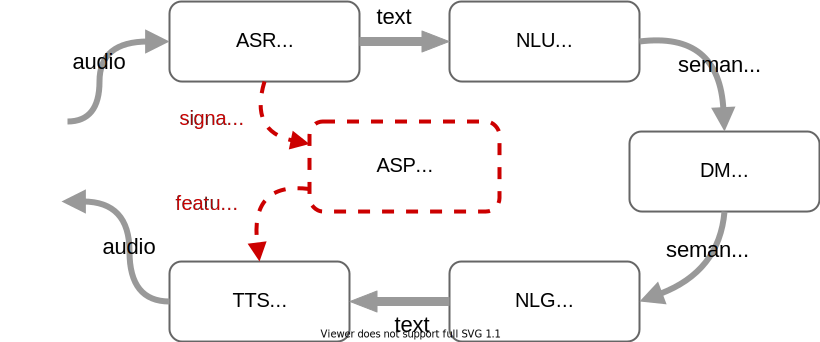
\includegraphics[width=\linewidth]{sds_architecture_ext_red}
	\caption[Proposed architecture for an accommodative \acl{sds}]
		{Suggested architecture for an accommodative \acl{sds} (cf.\ base architecture in \cref{fig:sds_architecture}).
		The added \acs{asp} module and its links from the \acs{asr} and to the \acs{tts} modules are colored in red.}
	\label{fig:adaptation_module_architecture}
\end{figure}

\subsection{Speech manipulation}
\label{subsec:speech_manipulation}

Although the \ac{asp} module is not responsible for the synthesis of the system's speech output, it is important to show that it provides relevant information for speech synthesis.
This is especially important since the synthesis, along with the required changes for expressing accommodation, need to be applied \emph{in real-time} and cannot be learned offline prior to an interaction.
The examples given here focus on segmental features, because real-time manipulation techniques for them are less common than for supra-segmental features like \ac{f0} and \ac{ar}.
For segmental features, modifications are applied to specific sounds occurring within short timespans, as oppose to supra-segmental features where longer segments and even an entire utterance are influenced.
The challenge is, therefore, to apply these modifications with smooth transition from and to the surrounding surrounding segments and without creating artifacts.

\todo[inline]{if have time, also create an example of the first approach}
The manipulation itself can be done either post-hoc on the audio signal itself or as part of the synthesis.
The first approach relies on signal processing techniques that can be applied on the \ac{tts} output to achieve the desired modification.
For this, the timespans of the target feature must be acquired from the \ac{tts} engine to detect the part in the signal that needs to be modified.
Then, the appropriate process needs to be applied.
For example, changing the format frequencies to manipulate vowel quality, shortening a segment to achieve \textipa{[@]} elision, etc.
Many of the manipulations can be done based on the source-filter theory \citep{Fant1970acoustic}, but any type manipulation would need to be written manually and run after the \ac{tts} finished generating the speech signal.
The second approach relies on the \ac{tts} model to be able to capture the variations of the target feature.
This might be difficult, especially for non-categorical features with relatively subtle changes.
The model would need to be trained on a dataset that contains the feature's variations.
As with any learning task, it is not guaranteed that the model will correctly learn them or be able to apply them correctly every time.
On the other hand, if works property, this approach is more robust and should create fewer artifacts, because direct manipulation of the signal is avoided.
However, direct manipulation might be more accurate and offer direct control over the change in the signal which might not be achieved using a pre-trained model.
These trade-off are an important consideration when choosing an approach, which might depend on the requirements of the application in question.

Both approaches were tested to realize accommodation changes.
The first with the feature \textipa{[E:]} vs.\ \textipa{[e:]} which requires a manipulation in the vowel space continuum, and the second with the categorical feature \emph{\textipa{[\c{c}]} vs.\ \textipa{[k]}}.
The source-filter manipulation was done as follows:
First, the formant contours were extracted from the audio signal.
this was done by computing the LPC coefficients with the algorithm by Burg, as given by \citet{Press1989numerical}.
One value was extracted per formant every \SI{6}{\milli\second} with linear interpolation for missing values.
Then, the first and second formants of the vowel target were changed separately using overlap-add \citep{Hamon1989diphone}.
The changes were based on the respective means of the formants in the duration of the target vowel, while taking the overall contour into account.
Finally, The original signal was used as the source and was filtered by the manipulated formant contours, resulting in a new speech signal that differs from the original only by the target vowel's segment.
The second approach was done with neural synthesis using Tacotron\footnote{Tacotron2 architecture based on the implementation in the repository \url{https://github.com/NVIDIA/tacotron2}} \citep{Shen2018natural}, which is trained to generate spectral information directly from textual input, and the neural vocoder WaveGlow \citep{Prenger2019WaveGlow}.
To capture the categorical allophonic variance, the system was trained on \emph{phonemic} input (as opposed to usual grapheme-based representations).
For this, the neutral voice subset of the PAVOQUE dataset\footnote{\url{https://github.com/marytts/pavoque-data}} \citep{Steiner2013pavoque} was used, which comprises $\sim$\SI{5.8}{\hour} of speech.
The phonetic transcriptions were done automatically based on the transcriptions provided with the dataset and were manually verified and corrected.
After training, the model was able to generate synthesized speech based on an input of an arbitrary phoneme sequence.
This opens many possibilities, one of them is alternating between \textipa{[\c{c}]} and \textipa{[k]} to express the variation of this feature.
It is important to note that the other-category variant of a word was not included in any dictionary and was not seen by the model during training \citep[and see][for more details]{Raveh2021ICASSP}.
\todo{remove ICASSP reference if it's not accepted}
\Cref{fig:spectrogram_ic_ik} shows an example of an original sentence (pronounced with \textipa{[\c{c}]} sounds) and its manipulated form (with \textipa{[k]} sounds).
%
\begin{landscape}
	\begin{figure}[t]
		\centering
		\vspace*{-2cm}
		\hspace*{-3cm}
		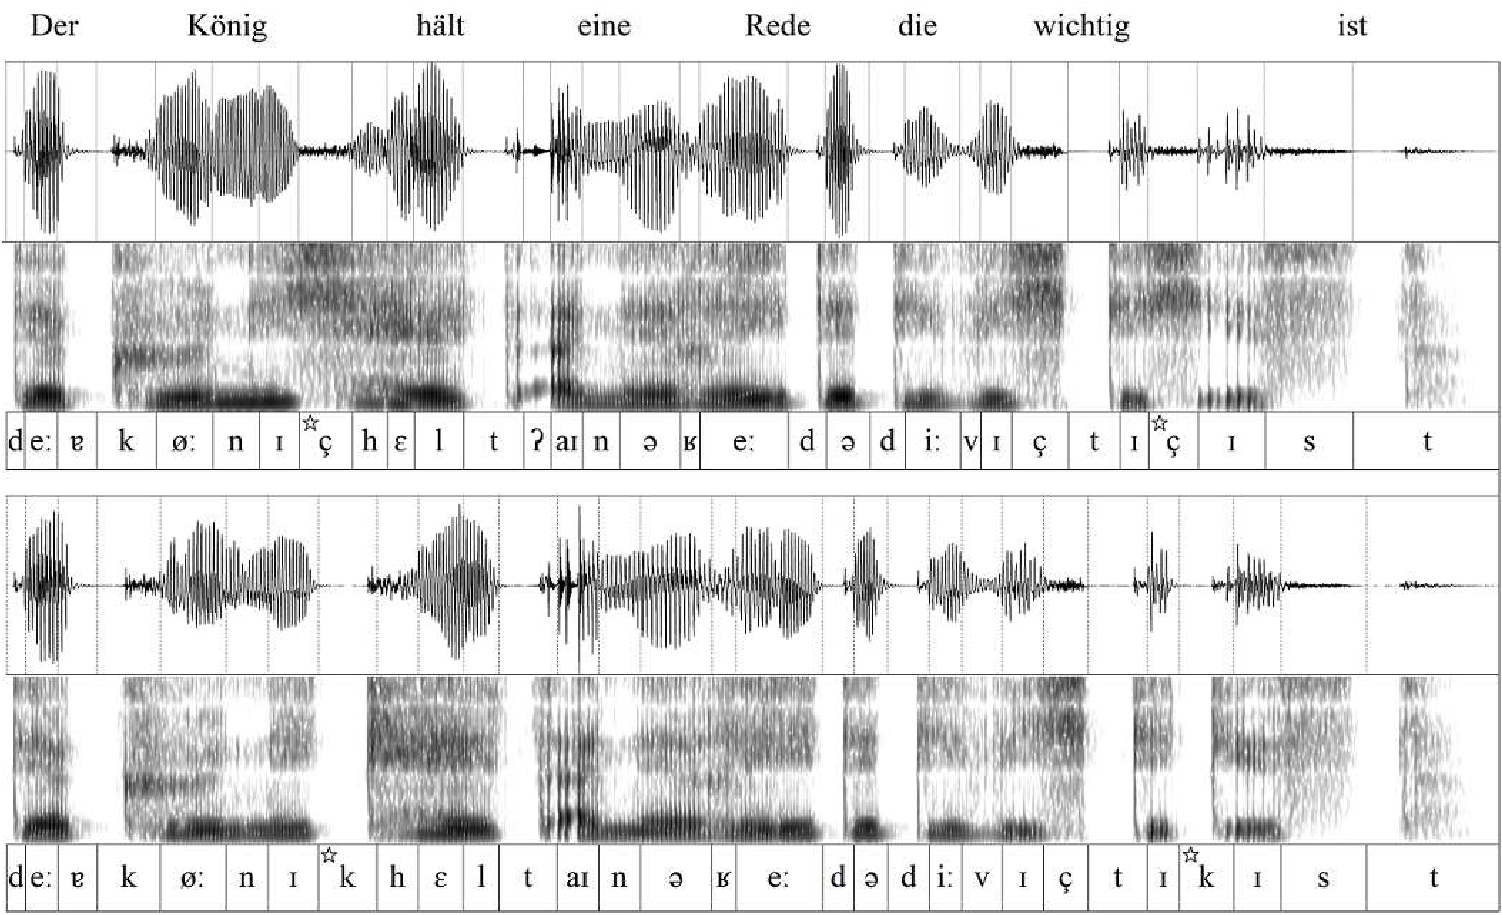
\includegraphics[width=1.5\textwidth]{ic_ik_manipulation_starred}
		\caption[Oscillograms and spectrograms of categorical manipulation speech outputs]
			{Oscillograms and spectrograms of the words \emph{\enquote{König}} (king) and \emph{\enquote{wichtig}} (important) pronounced originally with \textipa{[\c{c}]} (top), which were changed into \textipa{[k]} (bottom).
			The modified segments are marked with a star above the phoneme symbol in the transcriptions, and it can be seen that no artifacts were introduced in any other segment.
			The vertical lines show the phonemic segmentation.
			(note that the segments are not perfectly aligned in the two productions).
			The x-axis shows the chronological phonetic transcription over time (\SI{2.34}{\second} in total) and the spectrograms' y-axes show the frequencies up to \SI{5000}{\hertz}.}
		\label{fig:spectrogram_ic_ik}
	\end{figure}
\end{landscape}